% Preambulo -> 
\documentclass[11pt, a4paper]{article}
\usepackage{graphicx} % Required for inserting images
\usepackage{float} % Para agregar imagen en el lugar
\usepackage{tikz} % Insertar gráficos
\usepackage{amsmath}% Para usar ecuaciones
\usepackage{siunitx} % para angulos
\usepackage{wrapfig} % Imagen con texto al lado

% Título del documento
\title{Ecuaciones de latitud}
\author{Ian Chen}
\date{4th June 2024}

%--------------------
\begin{document}

% \begin{abstract}
%     Ecuaciones de latitud según la ubicación de la estrella.\\
%     Hecho con \LaTeX.
% \end{abstract}

\section{Hemisferio Sur}
% -----caso 1-
\subsection{Caso 1}
Cuando la estrella se encuentra entre Ecuador Celeste y Horizonte.
\vspace{0.5cm}

\begin{figure}[H]
    \centering
    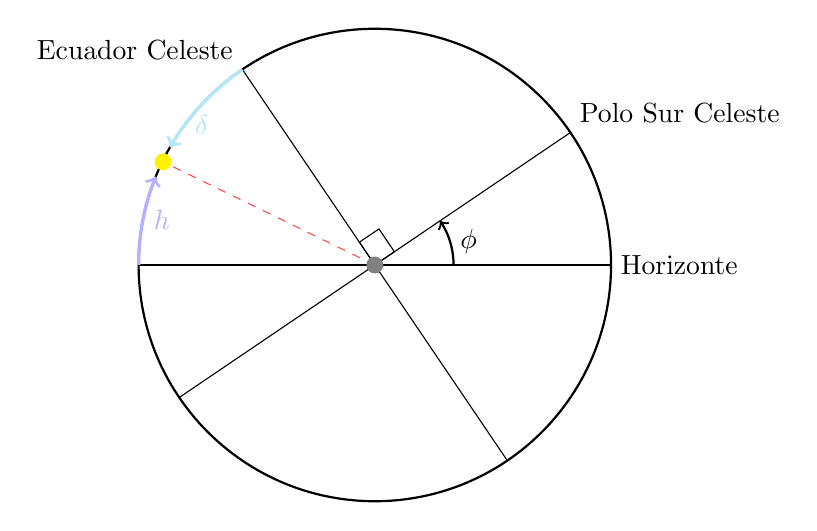
\begin{tikzpicture}
    % Circunferencia
    \draw[black, thick] (0,0) circle (3);
    
    % Rectas / Líneas
    \draw[black, thin] (-3, 0) -- (3, 0) node[anchor=west]{Horizonte};
    \draw[black, thin] (-2.48, -1.68) -- (2.48, 1.68) node[anchor=south west]{Polo Sur Celeste};
    \draw[black, thin]  (1.68, -2.48) -- (-1.68, 2.48)  node[anchor=south east]{Ecuador Celeste};
    \draw[red!70, dashed] (0,0) -- (-2.69, 1.31);

    % Arcos
    \draw[cyan!30, very thick, ->] (-1.68, 2.48) arc (124:150:3) node[midway, below]{$\delta$};
    \draw[blue!30, very thick, ->] (-3, 0) arc (180:158:3) node[midway, right]{$h$};
    \draw[black, thick, ->] (1, 0) arc (0:34:1) node[midway, right]{$\phi$};
    
    % Cuadrados
    \draw[black, thin, rotate around={34:(0,0)}] (0,0) rectangle (0.3, 0.35);

    % Puntos
    \filldraw[fill=black!50, draw=black!50] (0,0) circle (0.1);
    \filldraw[fill=yellow, draw=yellow] (-2.69,1.31) circle (0.1); % Estrella en angulo 90º + 34º + 30º
\end{tikzpicture}
    \caption{Estrella entre Horizonte y Ecuador celeste}
    \label{fig:case-1}
\end{figure}
Deducción de la ecuación correspondiente para hallar latitud $\phi$ en este caso:
\begin{align*}
    |\phi| &= \ang{90}-(|h|+|\delta|)\\
    |\phi| &= \ang{90}-|h|-|\delta| \\
    -\phi &= \ang{90} - h - \delta \\
    \phi &= -\ang{90} + h + \delta \\
    \phi &= h + \delta - \ang{90}
\end{align*}

\newpage
%%%%%%%%%%%%%%%%%%%%%%%%%%%%%%%%
% caso 2
\subsection{Caso 2}
Cuando la estrella se encuentra entre Ecuador Celeste y Polo Sur Celeste.
\vspace{1cm}
\begin{figure}[H]
    \centering
    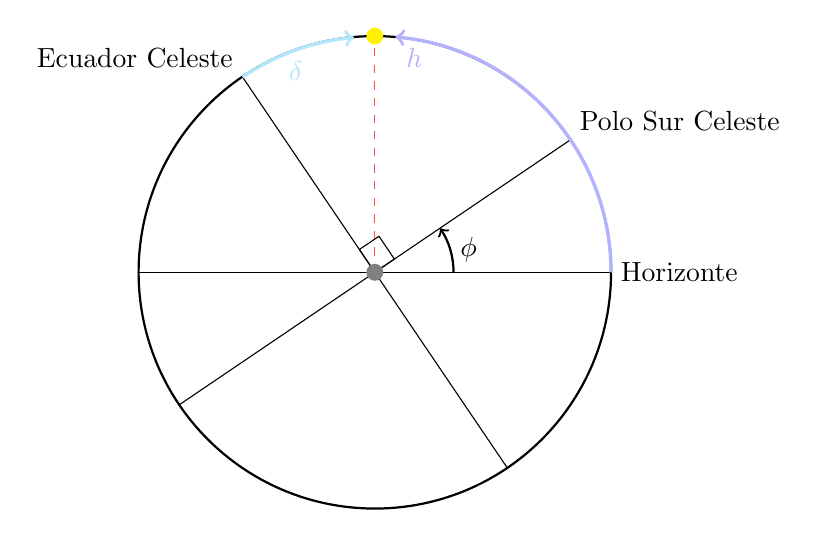
\begin{tikzpicture}
    % Circunferencia
    \draw[black, thick] (0,0) circle (3);
    
    % Rectas / Líneas
    \draw[black, thin] (-3, 0) -- (3, 0) node[anchor=west]{Horizonte};
    \draw[black, thin] (-2.48, -1.68) -- (2.48, 1.68) node[anchor=south west]{Polo Sur Celeste};
    \draw[black, thin]  (1.68, -2.48) -- (-1.68, 2.48)  node[anchor=south east]{Ecuador Celeste};
    % Recta roja del punto
    \draw[red!70, dashed] (0,0) -- (0,3);

    % Arcos
    % Declinación
    \draw[cyan!30, very thick, ->] (-1.68, 2.48) arc (124:95:3) node[midway, below]{$\delta$};
    % Altura
    \draw[blue!30, very thick, ->] (3, 0) arc (0:85:3) node[anchor=north west]{$h$};
    % LATITUD (NO CAMBIAR)
    \draw[black, thick, ->] (1, 0) arc (0:34:1) node[midway, right]{$\phi$};
    
    % Cuadrados
    \draw[black, thin, rotate around={34:(0,0)}] (0,0) rectangle (0.3, 0.35);

    % Puntos
    % Centro
    \filldraw[fill=black!50, draw=black!50] (0,0) circle (0.1);
    % Estrella
    \filldraw[fill=yellow, draw=yellow] (0,3) circle (0.1); % Estrella en angulo 90º
\end{tikzpicture}
    \caption{Estrella entre Ecuador Celeste y Polo Sur Celeste}
    \label{fig:case-2}
\end{figure}

Deducción de la ecuación correspondiente para hallar latitud $\phi$ en este caso:
\begin{align*}
    |h|-|\phi| &= \ang{90}-|\delta| \\
    |\phi| &= -\ang{90}+|h|+|\delta| \\
    -\phi &= -\ang{90} + h - \delta \\
    \phi &= \ang{90} + \delta - h
\end{align*}

\newpage
%%%%%%%%%%%%%%%%%%%%%%%%%%%%%%%%
% caso 3
\subsection{Caso 3}
Cuando la estrella se encuentra entre Polo Sur Celeste y Horizonte.
\vspace{1cm}
\begin{figure}[H]
    \centering
    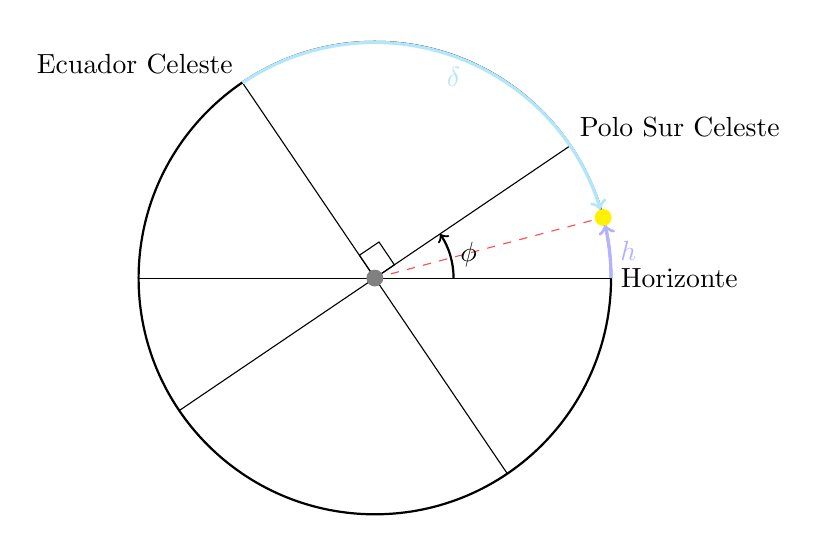
\begin{tikzpicture}
    % Circunferencia
    \draw[black, thick] (0,0) circle (3);
    
    % Rectas / Líneas
    \draw[black, thin] (-3, 0) -- (3, 0) node[anchor=west]{Horizonte};
    \draw[black, thin] (-2.48, -1.68) -- (2.48, 1.68) node[anchor=south west]{Polo Sur Celeste};
    \draw[black, thin]  (1.68, -2.48) -- (-1.68, 2.48)  node[anchor=south east]{Ecuador Celeste};
    % Recta roja del punto
    \draw[red!70, dashed] (0,0) -- (2.9,0.77);

    % Arcos
    % Declinación
    \draw[cyan!30, very thick, ->] (-1.68, 2.48) arc (124:17:3) node[midway, below]{$\delta$};
    % Altura
    \draw[blue!30, very thick, ->] (3, 0) arc (0:13:3) node[midway, right]{$h$};
    % LATITUD (NO CAMBIAR)
    \draw[black, thick, ->] (1, 0) arc (0:34:1) node[midway, right]{$\phi$};
    
    % Cuadrados
    \draw[black, thin, rotate around={34:(0,0)}] (0,0) rectangle (0.3, 0.35);

    % Puntos
    % Centro
    \filldraw[fill=black!50, draw=black!50] (0,0) circle (0.1);
    % Estrella
    \filldraw[fill=yellow, draw=yellow] (2.9,0.77) circle (0.1); % Estrella en angulo 90º
\end{tikzpicture}
    \caption{Estrella entre Horizonte y Polo Sur celeste}
    \label{fig:case-2}
\end{figure}

Deducción de la ecuación correspondiente para hallar latitud $\phi$ en este caso:
\begin{align*}
    |\phi|-|h|&= \ang{90}-|\delta| \\
    |\phi| &= \ang{90}+|h|-|\delta| \\
    -\phi &= \ang{90} + h - \delta \\
    \phi &= \delta - h - \ang{90}
\end{align*}

\newpage
\section{Hemisferio Norte}
%%%%%%%%%%%%%%%%%%%%%%%%%%%%%%%%
% caso 4
\subsection{Caso 4}
Cuando la estrella se encuentra entre Ecuador Celeste y Horizonte.
\vspace{1cm}
\begin{figure}[H]
    \centering
    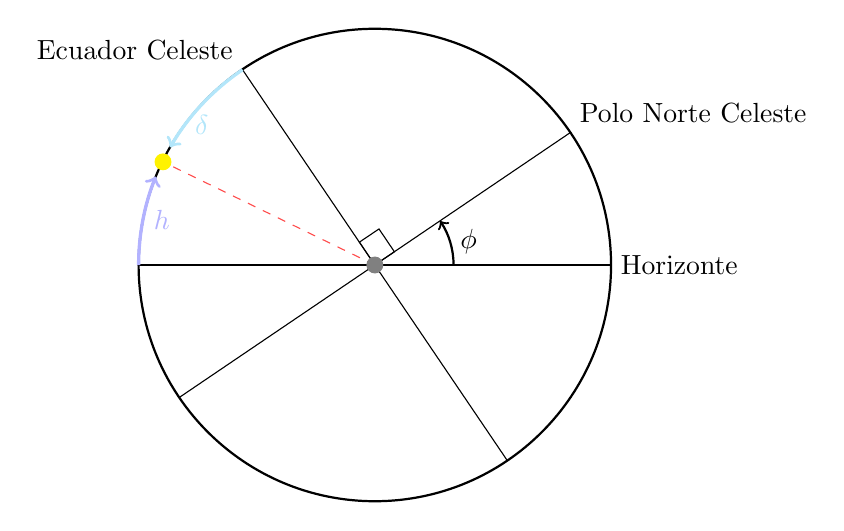
\begin{tikzpicture}
    % Circunferencia
    \draw[black, thick] (0,0) circle (3);
    
    % Rectas / Líneas
    \draw[black, thin] (-3, 0) -- (3, 0) node[anchor=west]{Horizonte};
    \draw[black, thin] (-2.48, -1.68) -- (2.48, 1.68) node[anchor=south west]{Polo Norte Celeste};
    \draw[black, thin]  (1.68, -2.48) -- (-1.68, 2.48)  node[anchor=south east]{Ecuador Celeste};
    \draw[red!70, dashed] (0,0) -- (-2.69, 1.31);

    % Arcos
    \draw[cyan!30, very thick, ->] (-1.68, 2.48) arc (124:150:3) node[midway, below]{$\delta$};
    \draw[blue!30, very thick, ->] (-3, 0) arc (180:158:3) node[midway, right]{$h$};
    \draw[black, thick, ->] (1, 0) arc (0:34:1) node[midway, right]{$\phi$};
    
    % Cuadrados
    \draw[black, thin, rotate around={34:(0,0)}] (0,0) rectangle (0.3, 0.35);

    % Puntos
    \filldraw[fill=black!50, draw=black!50] (0,0) circle (0.1);
    \filldraw[fill=yellow, draw=yellow] (-2.69,1.31) circle (0.1); % Estrella en angulo 90º + 34º + 30º
\end{tikzpicture}
    \caption{Estrella entre Horizonte y Ecuador celeste}
    \label{fig:case-1}
\end{figure}

Deducción de la ecuación correspondiente para hallar latitud $\phi$ en este caso:
\begin{align*}
    |\phi| &= \ang{90}-(|\delta| + |h|) \\
    |\phi| &= \ang{90}-|h|-|\delta| \\
    \phi &= \ang{90} - h + \delta
\end{align*}


\newpage
%______
% caso 5
\subsection{Caso 5}
Cuando la estrella se encuentra entre Ecuador Celeste y Polo Norte Celeste.
\vspace{1cm}
\begin{figure}[H]
    \centering
    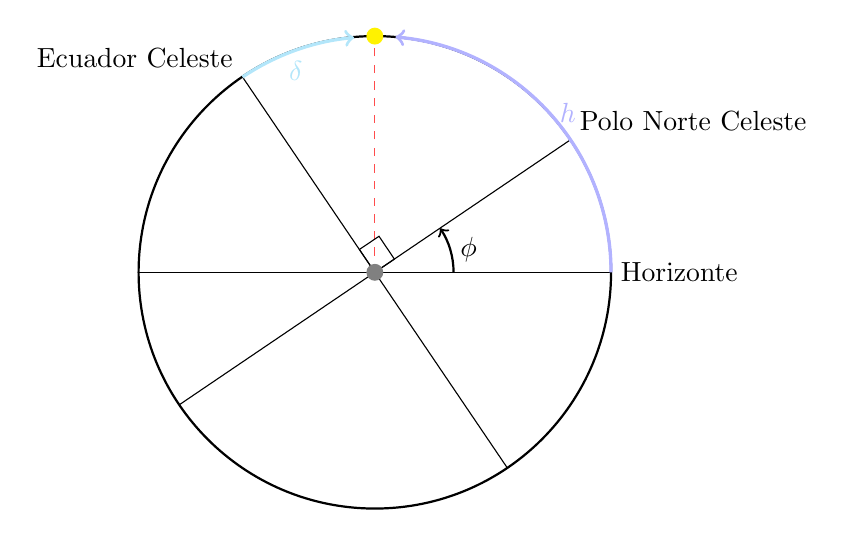
\begin{tikzpicture}
    % Circunferencia
    \draw[black, thick] (0,0) circle (3);
    
    % Rectas / Líneas
    \draw[black, thin] (-3, 0) -- (3, 0) node[anchor=west]{Horizonte};
    \draw[black, thin] (-2.48, -1.68) -- (2.48, 1.68) node[anchor=south west]{Polo Norte Celeste};
    \draw[black, thin]  (1.68, -2.48) -- (-1.68, 2.48)  node[anchor=south east]{Ecuador Celeste};
    % Recta roja del punto
    \draw[red!70, dashed] (0,0) -- (0,3);

    % Arcos
    % Declinación
    \draw[cyan!30, very thick, ->] (-1.68, 2.48) arc (124:95:3) node[midway, below]{$\delta$};
    % Altura
    \draw[blue!30, very thick, ->] (3, 0) arc (0:85:3) node[midway, right]{$h$};
    % LATITUD (NO CAMBIAR)
    \draw[black, thick, ->] (1, 0) arc (0:34:1) node[midway, right]{$\phi$};
    
    % Cuadrados
    \draw[black, thin, rotate around={34:(0,0)}] (0,0) rectangle (0.3, 0.35);

    % Puntos
    % Centro
    \filldraw[fill=black!50, draw=black!50] (0,0) circle (0.1);
    % Estrella
    \filldraw[fill=yellow, draw=yellow] (0,3) circle (0.1); % Estrella en angulo 90º
\end{tikzpicture}
    \caption{Estrella entre Ecuador Celeste y Polo Norte Celeste}
    \label{fig:case-5}
\end{figure}

Deducción de la ecuación correspondiente para hallar latitud $\phi$ en este caso:
\begin{align*}
    |h|-|\phi| &= \ang{90}-|\delta| \\
    |\phi| &= -\ang{90}+|h|+|\delta| \\
    \phi &= h + \delta -\ang{90}
\end{align*}


\newpage
%------------------
% Caso 6
\subsection{Caso 6}
Cuando la estrella se encuentra entre Horizonte y Polo Norte Celeste.
\begin{figure}[H]
    \centering
    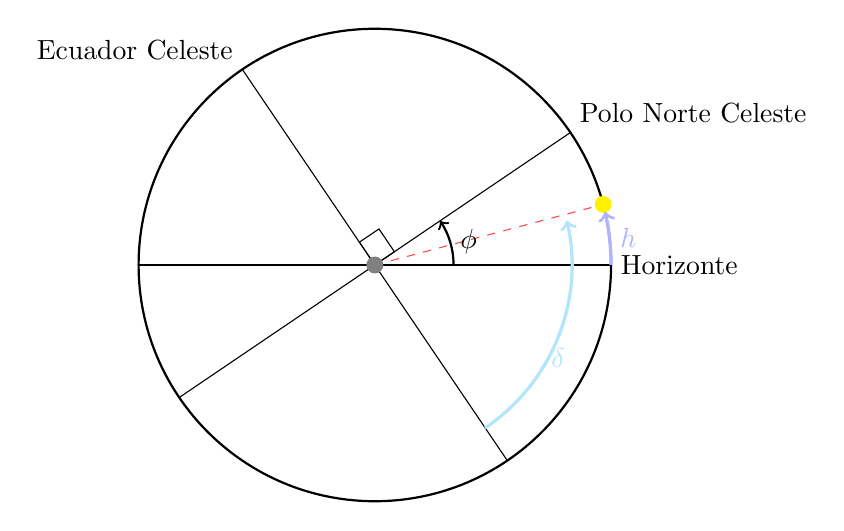
\begin{tikzpicture}
    % Circunferencia
    \draw[black, thick] (0,0) circle (3);
    
    % Rectas / Líneas
    \draw[black, thin] (-3, 0) -- (3, 0) node[anchor=west]{Horizonte};
    \draw[black, thin] (-2.48, -1.68) -- (2.48, 1.68) node[anchor=south west]{Polo Norte Celeste};
    \draw[black, thin]  (1.68, -2.48) -- (-1.68, 2.48)  node[anchor=south east]{Ecuador Celeste};
    % Recta roja del punto
    \draw[red!70, dashed] (0,0) -- (2.9,0.77);

    % Arcos
    % Declinación
    \draw[cyan!30, very thick, ->] (1.4, -2.07) arc (-56:13:2.5) node[midway, below]{$\delta$};
    % Altura
    \draw[blue!30, very thick, ->] (3, 0) arc (0:13:3) node[midway, right]{$h$};
    % LATITUD (NO CAMBIAR)
    \draw[black, thick, ->] (1, 0) arc (0:34:1) node[midway, right]{$\phi$};
    
    % Cuadrados
    \draw[black, thin, rotate around={34:(0,0)}] (0,0) rectangle (0.3, 0.35);

    % Puntos
    % Centro
    \filldraw[fill=black!50, draw=black!50] (0,0) circle (0.1);
    % Estrella
    \filldraw[fill=yellow, draw=yellow] (2.9,0.77) circle (0.1); % Estrella en angulo 90º
\end{tikzpicture}
    \caption{Estrella entre Horizonte y Ecuador celeste}
    \label{fig:case-6}
\end{figure}
Deducción de la ecuación correspondiente para hallar latitud $\phi$ en este caso:
\begin{align*}
    |\phi|-|h| &= \ang{90}-|\delta| \\
    |\phi| &= \ang{90}+|h|-|\delta| \\
    \phi &= \ang{90} + h - \delta
\end{align*}


\end{document}
